\documentclass[tikz,border=8pt]{standalone}
\usepackage{amsmath,amssymb}
\usetikzlibrary{arrows.meta,calc,decorations.markings}

\newcommand{\drawtri}[3]{%
  \draw[thick] (90:0.6) -- (210:0.6) -- (330:0.6) -- cycle;
  \node[font=\scriptsize] at (90:0.85) {#1};
  \node[font=\scriptsize] at (210:0.92) {#2};
  \node[font=\scriptsize] at (330:0.92) {#3};
}
\newcommand{\tcell}[3]{\node[font=\scriptsize] at (#1, #2) {#3};}

\begin{document}
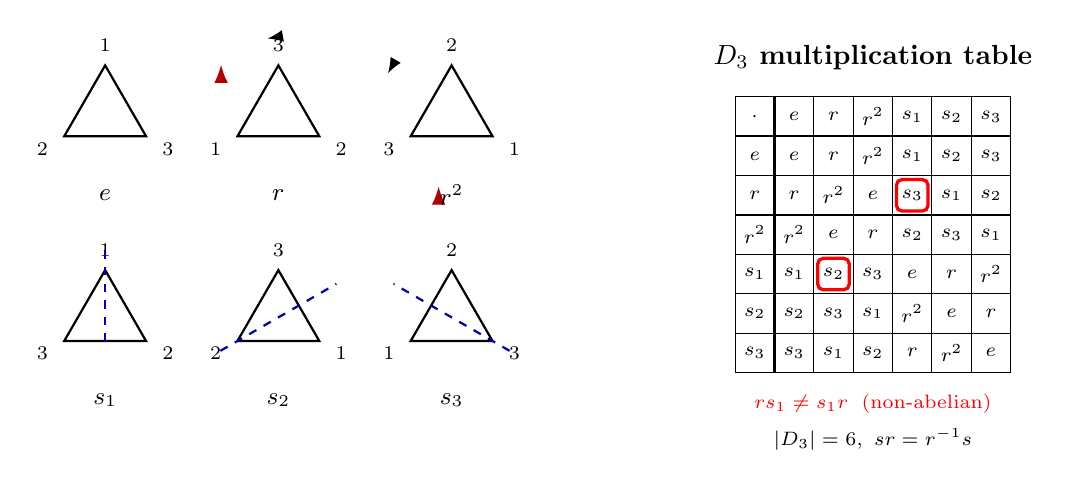
\begin{tikzpicture}[>=Latex]

  % Six elements (2 rows × 3 cols)
  \begin{scope}[shift={(0, 1.6)}]
    \drawtri{1}{2}{3}
    \node[font=\small\bfseries] at (0, -1.05) {$e$};
  \end{scope}
  \begin{scope}[shift={(2.2, 1.6)}]
    \drawtri{3}{1}{2}
    \draw[->, thick, red!70!black, decorate, decoration={markings, mark=at position 0.6 with {\arrow{>}}}] (40:0.95) arc (40:140:0.95);
    \node[font=\small\bfseries] at (0, -1.05) {$r$};
  \end{scope}
  \begin{scope}[shift={(4.4, 1.6)}]
    \drawtri{2}{3}{1}
    \draw[->, thick, red!70!black, decorate, decoration={markings, mark=at position 0.5 with {\arrow{>}}}] (40:0.95) arc (40:260:0.95);
    \node[font=\small\bfseries] at (0, -1.05) {$r^2$};
  \end{scope}

  \begin{scope}[shift={(0, -1.0)}]
    \drawtri{1}{3}{2}
    \draw[dashed, thick, blue!70!black] (0, 0.85) -- (0, -0.40);
    \node[font=\small\bfseries] at (0, -1.05) {$s_1$};
  \end{scope}
  \begin{scope}[shift={(2.2, -1.0)}]
    \drawtri{3}{2}{1}
    \draw[dashed, thick, blue!70!black] (210:0.85) -- (30:0.85);
    \node[font=\small\bfseries] at (0, -1.05) {$s_2$};
  \end{scope}
  \begin{scope}[shift={(4.4, -1.0)}]
    \drawtri{2}{1}{3}
    \draw[dashed, thick, blue!70!black] (330:0.85) -- (150:0.85);
    \node[font=\small\bfseries] at (0, -1.05) {$s_3$};
  \end{scope}

  % Multiplication table
  \begin{scope}[xshift=8.5cm, yshift=-1.7cm]
    \node[font=\bfseries] at (1.25, 4.0) {$D_3$ multiplication table};

    \draw[thin] (-0.5, 0) grid[step=0.5] (3.0, 3.5);
    \draw[thick] (-0.5, 3.0) -- (3.0, 3.0);
    \draw[thick] (0.0, 0)   -- (0.0, 3.5);

    \tcell{-0.25}{3.25}{$\cdot$}
    \tcell{0.25}{3.25}{$e$}
    \tcell{0.75}{3.25}{$r$}
    \tcell{1.25}{3.25}{$r^2$}
    \tcell{1.75}{3.25}{$s_1$}
    \tcell{2.25}{3.25}{$s_2$}
    \tcell{2.75}{3.25}{$s_3$}

    \tcell{-0.25}{2.75}{$e$}
    \tcell{-0.25}{2.25}{$r$}
    \tcell{-0.25}{1.75}{$r^2$}
    \tcell{-0.25}{1.25}{$s_1$}
    \tcell{-0.25}{0.75}{$s_2$}
    \tcell{-0.25}{0.25}{$s_3$}

    % e row
    \tcell{0.25}{2.75}{$e$}\tcell{0.75}{2.75}{$r$}\tcell{1.25}{2.75}{$r^2$}
    \tcell{1.75}{2.75}{$s_1$}\tcell{2.25}{2.75}{$s_2$}\tcell{2.75}{2.75}{$s_3$}
    % r row
    \tcell{0.25}{2.25}{$r$}\tcell{0.75}{2.25}{$r^2$}\tcell{1.25}{2.25}{$e$}
    \tcell{1.75}{2.25}{$s_3$}\tcell{2.25}{2.25}{$s_1$}\tcell{2.75}{2.25}{$s_2$}
    % r^2 row
    \tcell{0.25}{1.75}{$r^2$}\tcell{0.75}{1.75}{$e$}\tcell{1.25}{1.75}{$r$}
    \tcell{1.75}{1.75}{$s_2$}\tcell{2.25}{1.75}{$s_3$}\tcell{2.75}{1.75}{$s_1$}
    % s_1 row
    \tcell{0.25}{1.25}{$s_1$}\tcell{0.75}{1.25}{$s_2$}\tcell{1.25}{1.25}{$s_3$}
    \tcell{1.75}{1.25}{$e$}\tcell{2.25}{1.25}{$r$}\tcell{2.75}{1.25}{$r^2$}
    % s_2 row
    \tcell{0.25}{0.75}{$s_2$}\tcell{0.75}{0.75}{$s_3$}\tcell{1.25}{0.75}{$s_1$}
    \tcell{1.75}{0.75}{$r^2$}\tcell{2.25}{0.75}{$e$}\tcell{2.75}{0.75}{$r$}
    % s_3 row
    \tcell{0.25}{0.25}{$s_3$}\tcell{0.75}{0.25}{$s_1$}\tcell{1.25}{0.25}{$s_2$}
    \tcell{1.75}{0.25}{$r$}\tcell{2.25}{0.25}{$r^2$}\tcell{2.75}{0.25}{$e$}

    % highlight non-abelian: r·s_1 = s_3 vs s_1·r = s_2
    \draw[red, very thick, rounded corners=2pt] (1.55, 2.05) rectangle (1.95, 2.45);
    \draw[red, very thick, rounded corners=2pt] (0.55, 1.05) rectangle (0.95, 1.45);

    \node[font=\scriptsize, red] at (1.25, -0.4) {$rs_1\ne s_1 r$ \;(non-abelian)};
    \node[font=\scriptsize] at (1.25, -0.85) {$|D_3|=6,\ sr=r^{-1}s$};
  \end{scope}
\end{tikzpicture}
\end{document}
